\documentclass{article}
\usepackage[utf8]{inputenc}
\usepackage{geometry}
 \geometry{
 a4paper,
 total={170mm,257mm},
 left=20mm,
 top=20mm,
 }

\usepackage{hyperref}
 \usepackage{graphicx}
 \usepackage{titling}
 \usepackage{multirow}
 \usepackage{caption, subcaption}

\title{Performance comparison of functional and imperative $(a, b)$ trees}
\author{Nawat Ngerncham}
\date{April 2023}
 
 \usepackage{fancyhdr}
\fancypagestyle{plain}{%  the preset of fancyhdr 
    \fancyhf{} % clear all header and footer fields
    \fancyfoot[L]{\thedate}
    \fancyhead[L]{Applied Algorithms Project}
    \fancyhead[R]{\theauthor}
}
\makeatletter
\def\@maketitle{%
  \newpage
  \null
  \vskip 1em%
  \begin{center}%
  \let \footnote \thanks
    {\LARGE \@title \par}%
    \vskip 1em%
    %{\large \@date}%
  \end{center}%
  \par
  \vskip 1em}
\makeatother

\usepackage{lipsum}  
\usepackage{cmbright}

\begin{document}

\maketitle

\section{Background}

Functional interfaces for many data structures are becoming more and more common in 
modern programming languages as the functional style has many advantages, namely
its immutability leading to it being safer in concurent environments. However, the
big restriction of the functional style is that its data cannot be mutated---meaning
that in order to modify a data structure in many way, it would need to clone the entire
path from the root down to the node that is updated. This could be come very costly due
to the sheer number of memory allocations required. Thus, this project aimed to answer the following questions:

\begin{enumerate}
    \item Does the restriction imposed by the functional style hurt performance?
    \item In a functional $(a, b)$ tree, what would a good value for $a$ and $b$?
\end{enumerate}

\section{Progress Check}

Since there were a few to-dos in the proposal, let us first have a look at what was
achieved and what were not.

\begin{itemize}
    \item Implement an $(a, b)$ tree in an imperative and functional style such that 
        $a$ and $b$ can be easily changed:
        \begin{itemize}
            \item  Due to my stubbornness of trying to
                implement this in Rust, I wasted a lot of time and ended up changing to
                C++ last minute so the tree actually implemented in the experiments are
                $B$-trees instead of true $(a, b)$ trees. Additionally, these $B$-trees
                only support insertion and not deletion. However, an imperative $B$-tree
                and a functional $B$-tree that uses full path cloning are implemented and
                used in benchmarking. These trees also support an easy way to change $b$
                since it takes $b$ in its constructor.
        \end{itemize}

    \item Compare the performance of both versions.
        \begin{itemize}
            \item The results and discussion are further below.
        \end{itemize}

    \item Find the \textit{theoretical best (if possible)} for the value of $a$ and $b$
        for the purely functional style.
        \begin{itemize}
            \item Since the tree implemented is a $B$-tree instead of an $(a, b)$ tree, the only
                thing we can optimize for is just $b$. The discussion for this is further below.
        \end{itemize}
\end{itemize}

\section{Theoretical Discussion}

Since any insertion/deletion operation will, in the worst case, require creating a clone of the
full path from the root down to the leaf, we will be mainly focusing on the theoretical bound since
so we can minimize the amount of \textit{things} we need to clone when modifying the tree and
optimizing for cache hits is more useful when we are only updating a single node.

To minimize the amount of \textit{things} we need to clone, let us first model it as a function:
$$ f(n) = b\log_{b/2}n $$
where $n$ is the number of key(-value pair)s in a tree and $b$ is the maximum number of
key(-value pair)s per node. This comes from the fact that the height of the tree is at most
$\log_{a}n$ where we let $a$ be $b/2$ and we need to copy the $b$ elements in a single node.
Minimizing this gives us $b = 5.437$ using the minimize function
from SciPy. Since $b$ must be an integer, we try for $b = 5$ and $6$.

\section{Experiment Setup}

Firstly, the trees are implemented using the imperative and functional style. For the map
version, it is a map from an integer to a string. For the sequence, it is a sequence of
integers. Then, a sequence of integers (and keys) are randomly generated and inserted into
each implementation of the tree. rdtsc is used to time each insertion.

\section{Results and Discussion}

\begin{figure}[h]
    \centering
    \begin{subfigure}[b]{0.6\textwidth}
        \centering
        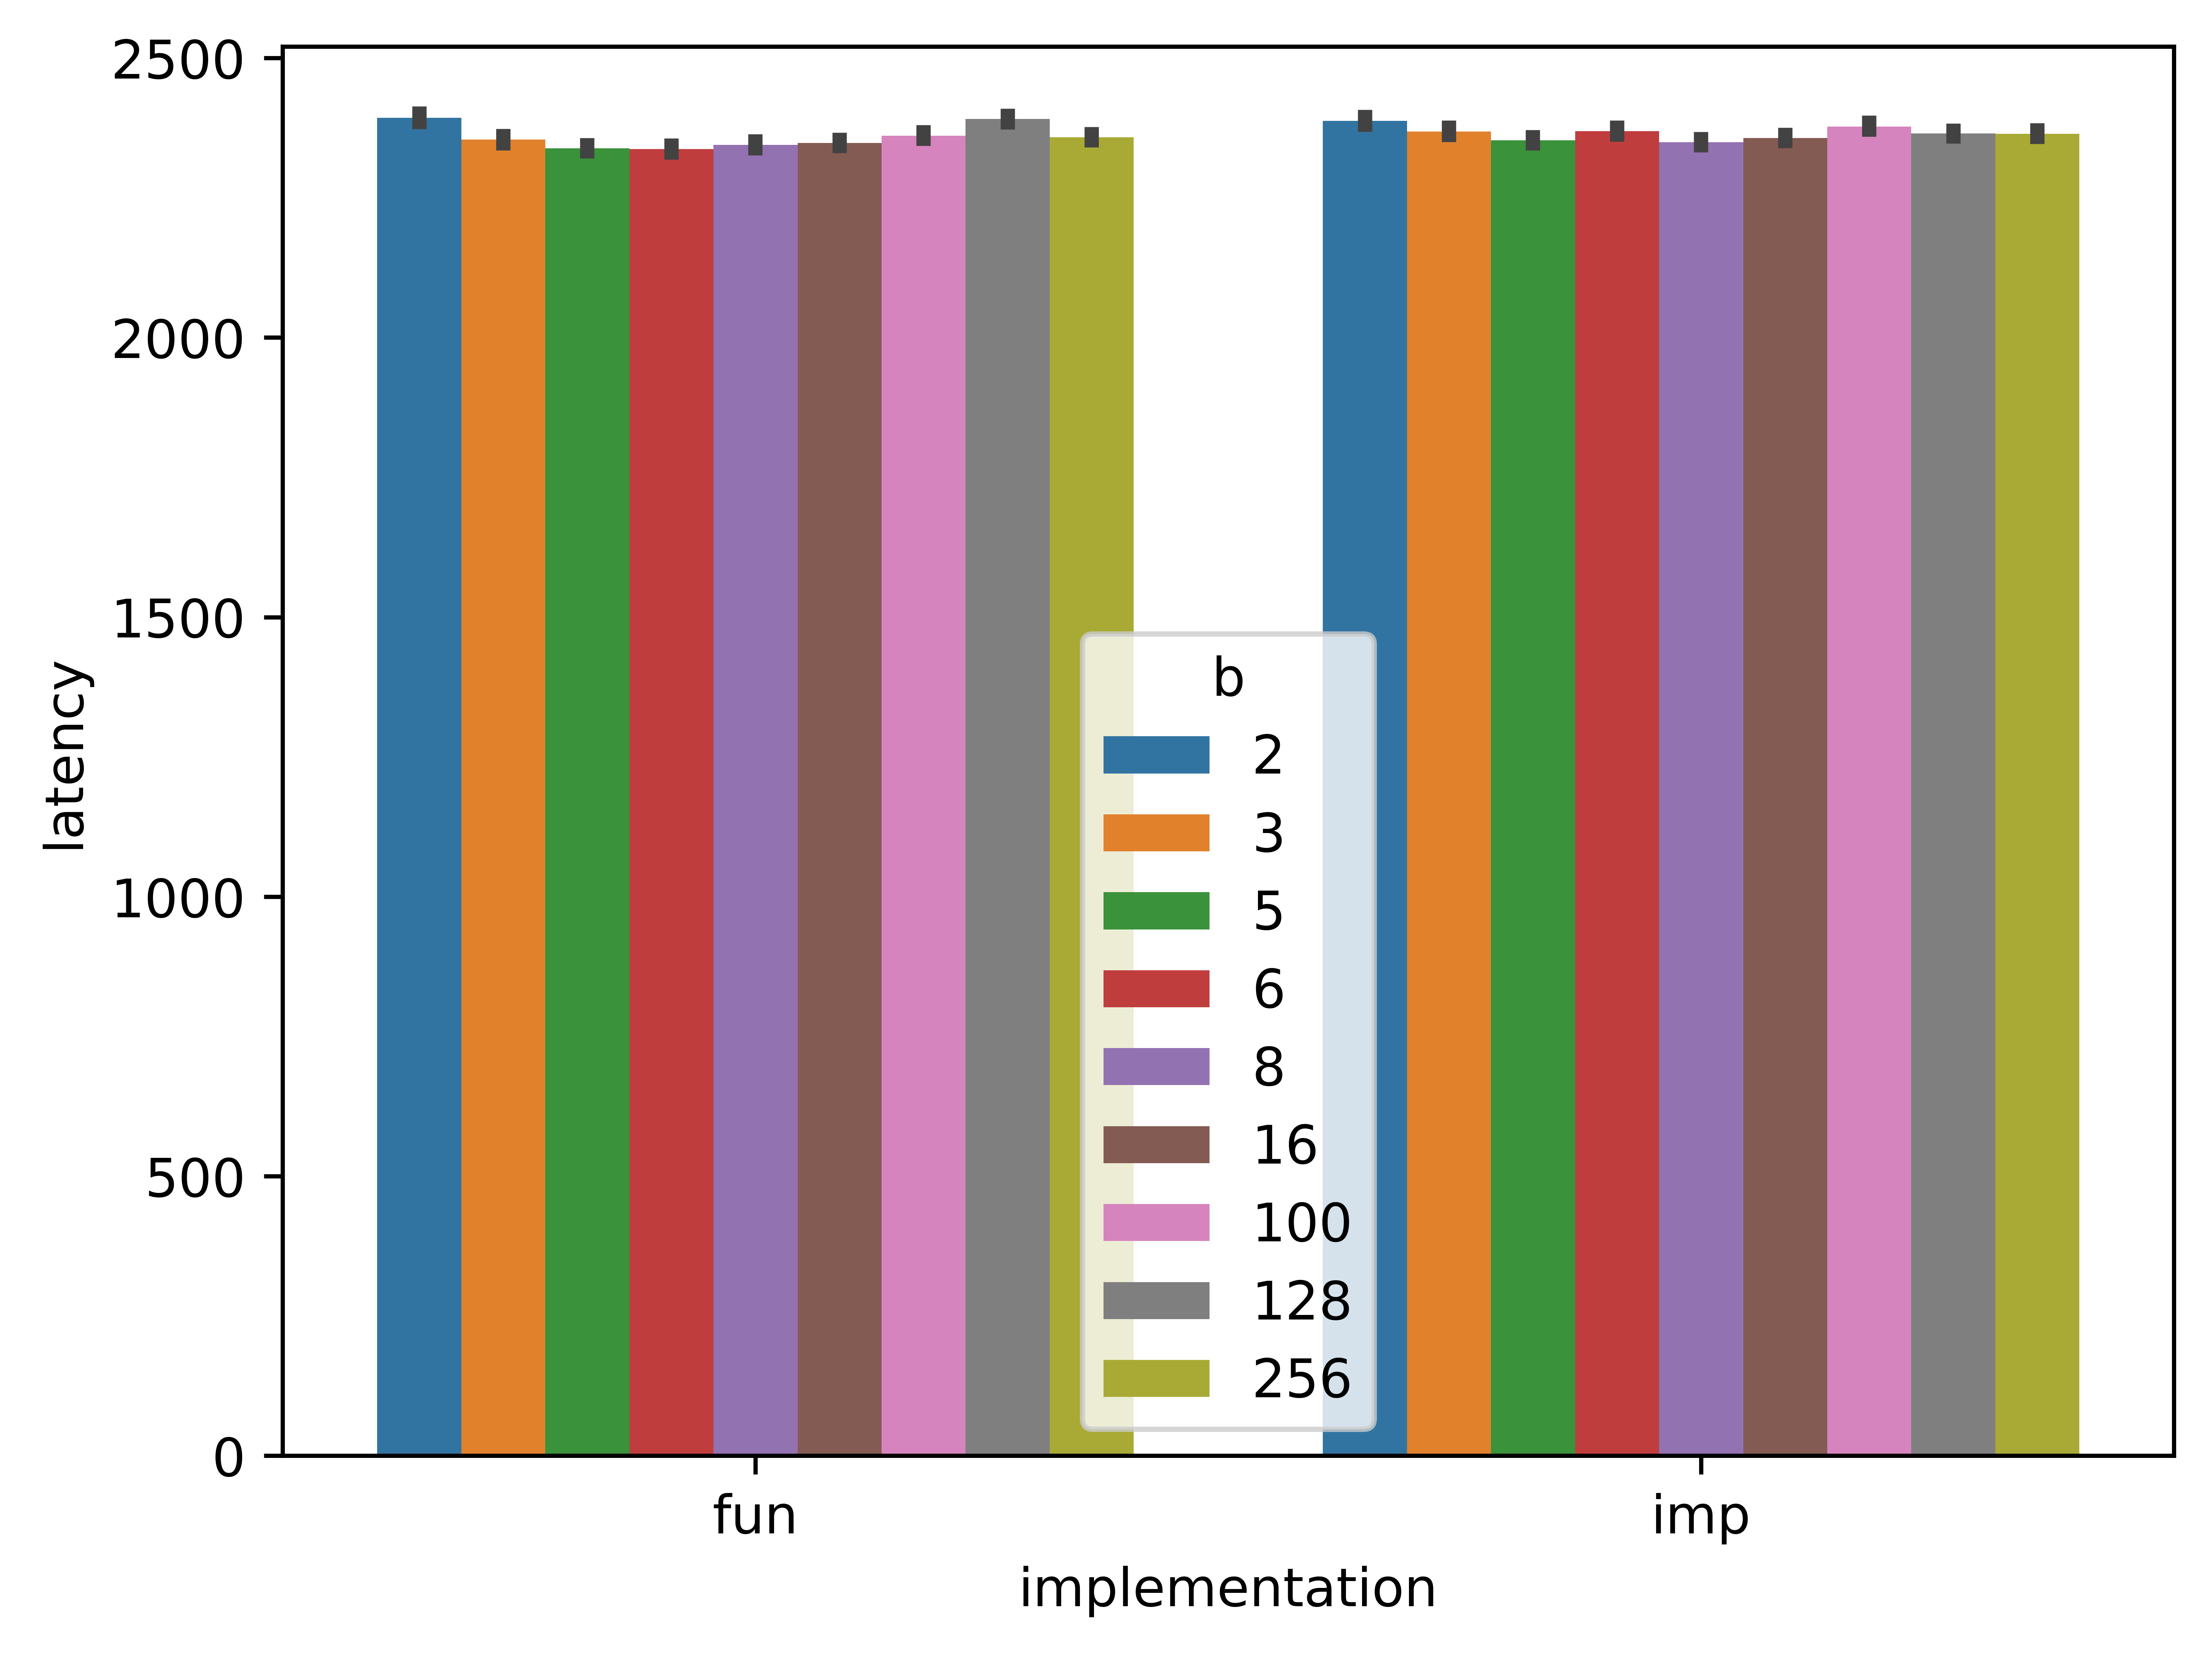
\includegraphics[width=\textwidth]{average-map.png}
        \caption{Average latency}
    \end{subfigure}
    % \hfill
    \begin{subfigure}[b]{0.3\textwidth}
        \centering
        \begin{tabular}{llr}
             &  & latency \\
            b & implementation &  \\
            \multirow[c]{2}{*}{2} & fun & 5093.050000 \\
             & imp & 4847.000000 \\
            \multirow[c]{2}{*}{3} & fun & 4723.050000 \\
             & imp & 4736.000000 \\
            \multirow[c]{2}{*}{5} & fun & 4699.000000 \\
             & imp & 4662.000000 \\
            \multirow[c]{2}{*}{6} & fun & 4625.000000 \\
             & imp & 4625.000000 \\
            \multirow[c]{2}{*}{8} & fun & 4575.050000 \\
             & imp & 4551.000000 \\
            \multirow[c]{2}{*}{16} & fun & 4514.000000 \\
             & imp & 4551.000000 \\
            \multirow[c]{2}{*}{100} & fun & 4514.000000 \\
             & imp & 4551.000000 \\
            \multirow[c]{2}{*}{128} & fun & 4588.000000 \\
             & imp & 4514.000000 \\
            \multirow[c]{2}{*}{256} & fun & 4588.000000 \\
             & imp & 4514.000000 \\
        \end{tabular}
        \caption{99-percentile latency}
    \end{subfigure}
    \caption{Results for maps}
    \label{fig:map}
\end{figure}

\begin{figure}
    \centering
    \begin{subfigure}[b]{0.6\textwidth}
        \centering
        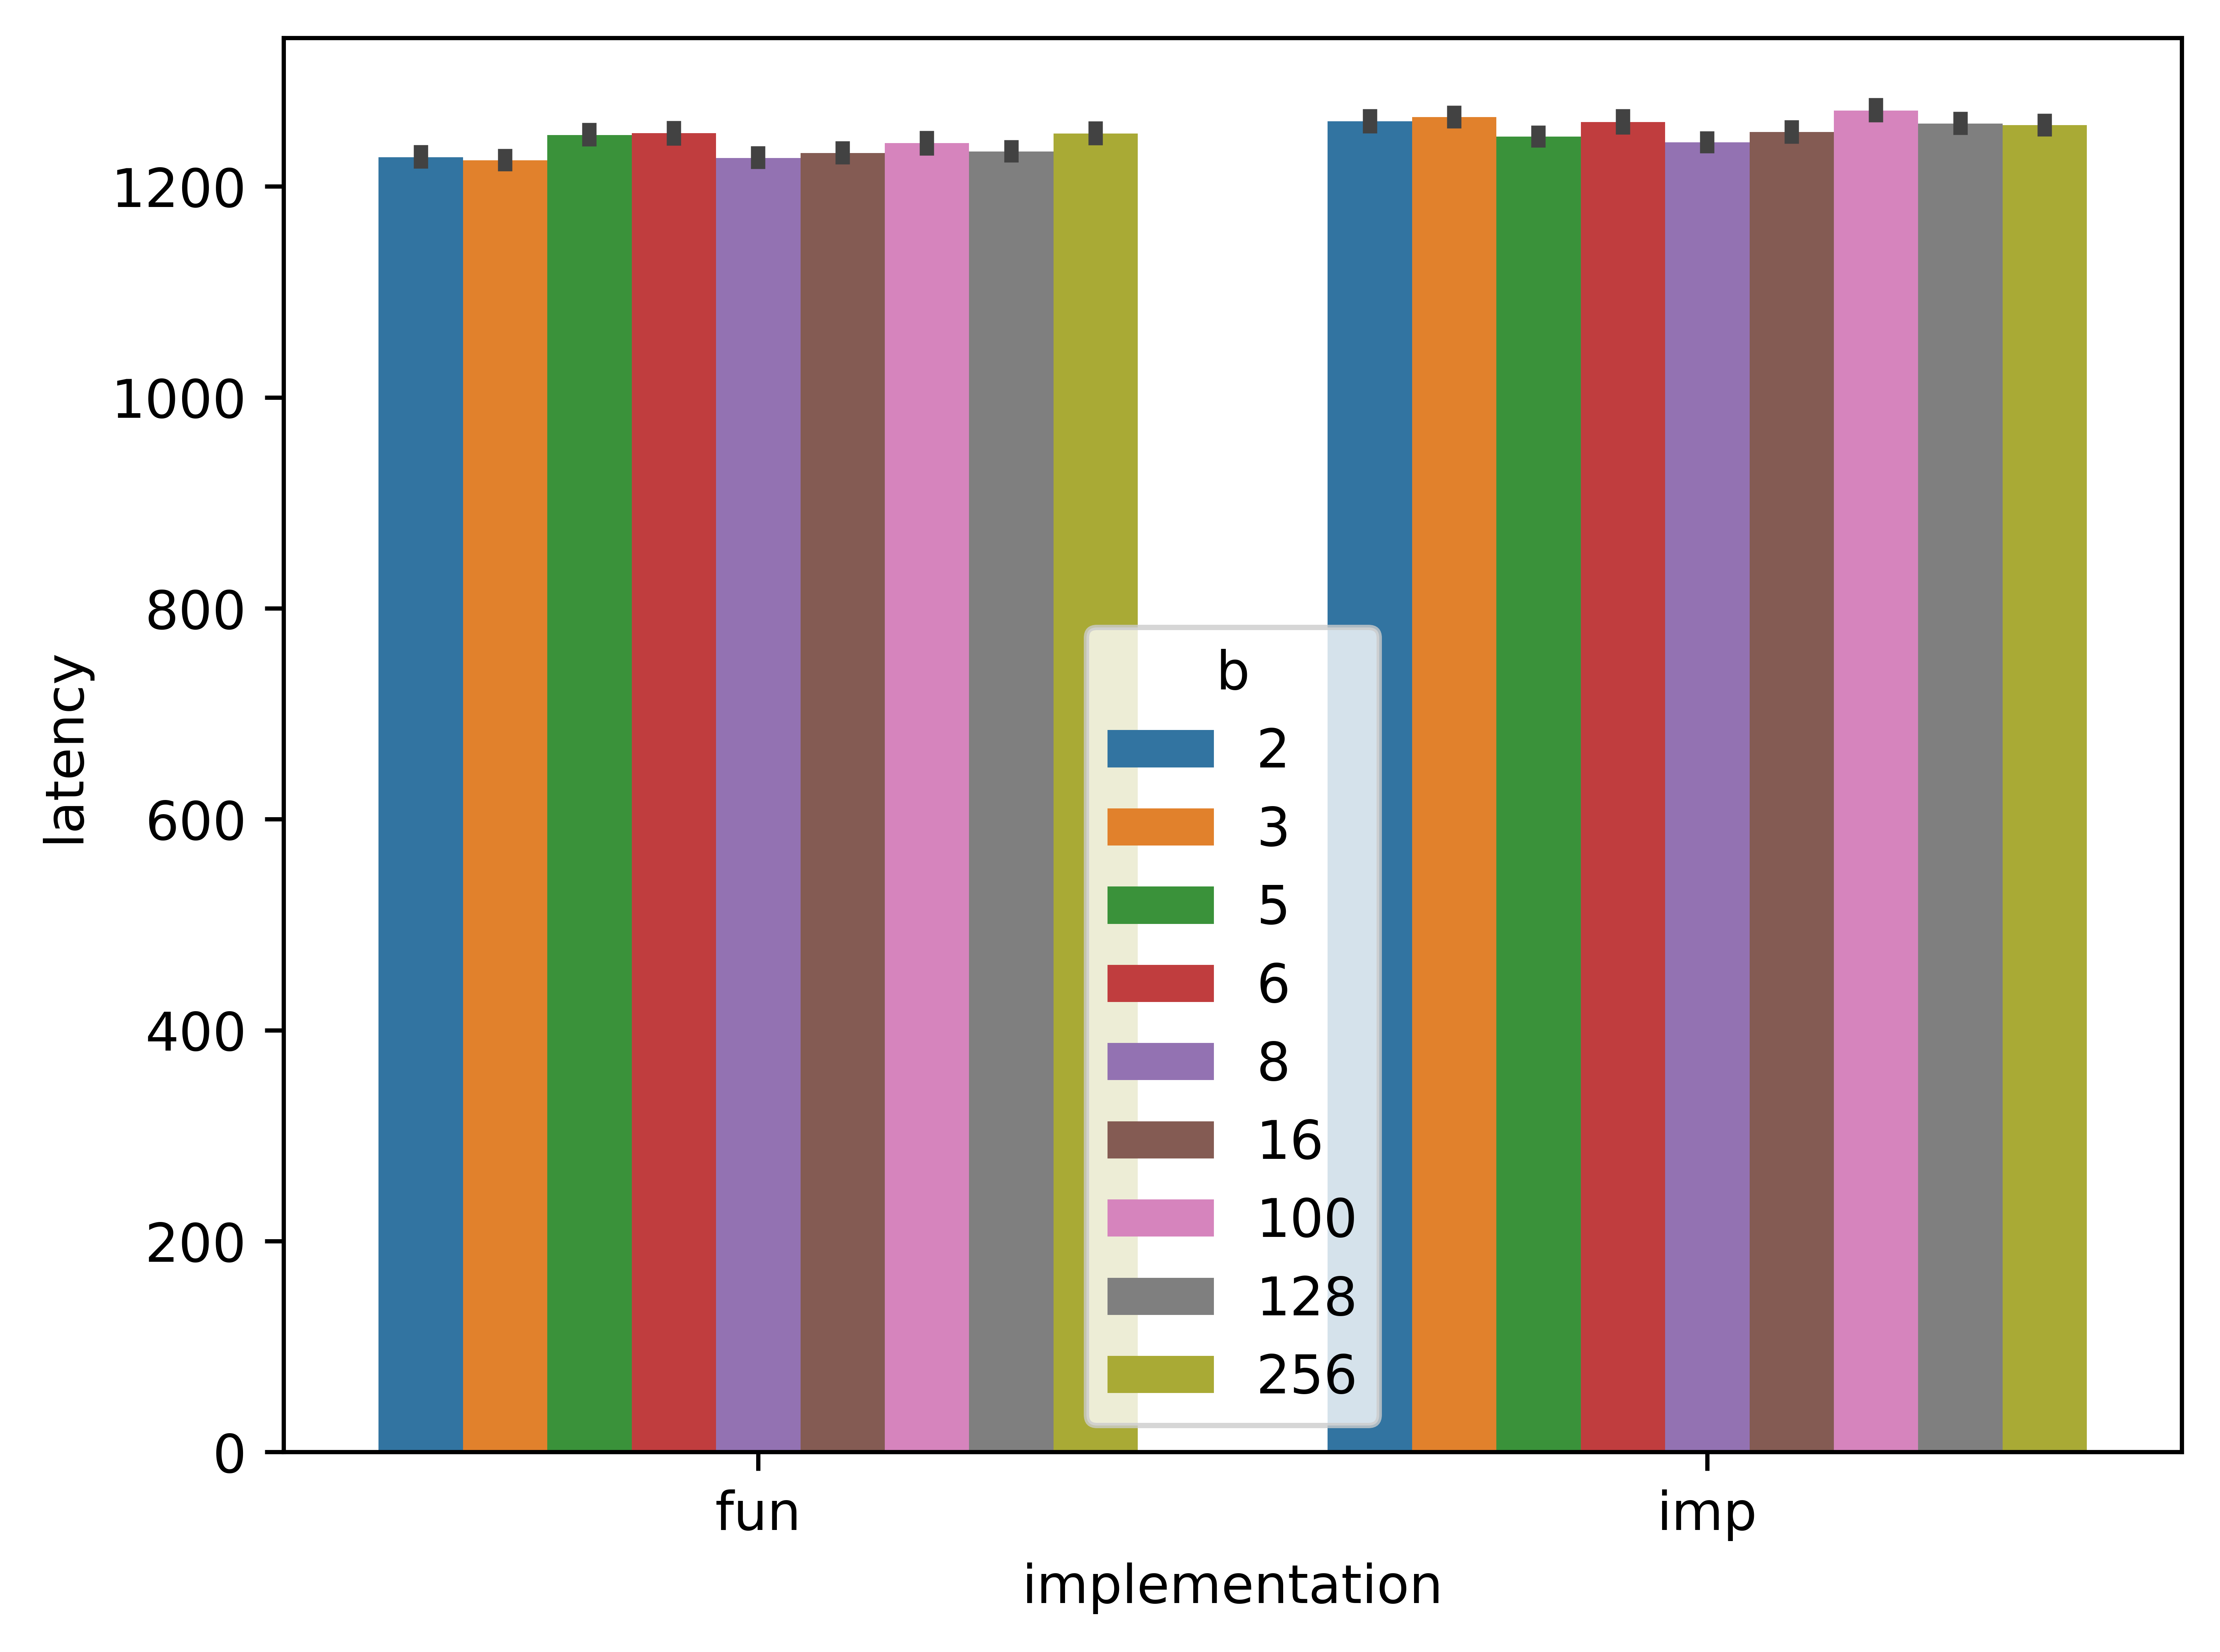
\includegraphics[width=\textwidth]{average-seq.png}
        \caption{Average latency}
    \end{subfigure}
    \begin{subfigure}[b]{0.3\textwidth}
        \centering
        \begin{tabular}{llr}
             &  & latency \\
            b & implementation &  \\
            \multirow[c]{2}{*}{2} & fun & 3293.000000 \\
             & imp & 3256.000000 \\
            \multirow[c]{2}{*}{3} & fun & 3145.000000 \\
             & imp & 3256.000000 \\
            \multirow[c]{2}{*}{5} & fun & 3256.000000 \\
             & imp & 3293.000000 \\
            \multirow[c]{2}{*}{6} & fun & 3293.000000 \\
             & imp & 3293.000000 \\
            \multirow[c]{2}{*}{8} & fun & 3182.000000 \\
             & imp & 3256.000000 \\
            \multirow[c]{2}{*}{16} & fun & 3182.000000 \\
             & imp & 3219.000000 \\
            \multirow[c]{2}{*}{100} & fun & 3256.000000 \\
             & imp & 3219.000000 \\
            \multirow[c]{2}{*}{128} & fun & 3256.000000 \\
             & imp & 3293.000000 \\
            \multirow[c]{2}{*}{256} & fun & 3293.000000 \\
             & imp & 3219.000000 \\
        \end{tabular}
        \caption{99-percentile}
    \end{subfigure}
    \caption{Results for sequences}
    \label{fig:sequence}
\end{figure}

The results of maps are shown in Figure \ref{fig:map} and the results of sequences are shown in
Figure \ref{fig:sequence}.

On average, it seems that both implementation of the $B$-tree sequence and map perform 
about the same. This is good news since it means that an average
user would not be able discern the difference between the two. This is quite surprising given that
the functional style requires copying the entire path from the root down to the modified node
while the imperative style only needs to do the insertions in the leaf nodes. There also seems
to be no difference between the different values of $b$.

The 99-percentile tells the same story. Both the functional and imperative implementations of the
sequence and map have their respective 99-percentile within around 100 cycles of each other. While
that may seem like a lot, but to an average user, it would not be that noticable.

The most surprising result to me must be the difference in latency between the different values
of $b$, or specifically the lack thereof.
While the average latency seems to dip a bit lower than the rest when $b = 5$ and $6$ for
the functional implementation of map, this could just be due to sheer luck since the experiments
are only run for a few times which could not show that this is significant. Additionally since,
in the case of functional sequence, they seem to perform the worst when $b = 5$ or $6$.
Still, it is surprising that $b$ does not have that much effect on the latency.

\subsection*{Answering an ongoing in-class question}

Here is a (naive) hypothesis on why binary trees are still used to implement ordered
maps in many programming languages rather than a $B$-tree even though it should be more cache
efficient.

As seen in the results, the implementation and value of $b$ barely has any effect
on the performance. Since a binary tree is simply a $(1, 2)$ tree, the performance will not be
so much different for different values of $a$ and $b$. Additionally, re-implementing the ordered
maps using $(a, b)$ or $B$-trees could also be costly since a lot of existing code base would
need to be modified especially since it would not have the same level of optimization as the
existing binary trees as it has been worked on for a very long time.

Furthermore, the cache efficiency of $B$-trees may still be roughly the same as binary trees.
Consider that for a single key in a map, each node requires enough space for three
vectors of addresses (key, value, children) and each memory is 64 bits in a modern computer.
This means that we will need at least 24 bytes per node. 
Recall that a cache line is typically 32, 64, or 128 bytes. For a map, we would be able to fit
1, 2, and 4 nodes in a cache line at a time respectively. 
Suppose that we want to support any type of data, we would need to store the addresses of the keys,
values, and children which takes up quite a lot of space. As a result, typical binary tree node
could already be taking up the entire cache line already if it is only 32 bytes so making it any 
bigger would not be any more cache efficient if we want to support every computer---including
that those whose cache line size is 32 bytes.

Still, since the results of this experiment could be affected by so many factors---especially
bad implementation---this is no definitive answer to why binary trees are still preferred over
$B$-trees in many languages. Another reason could just be that my cache efficiency analysis is
super off-point, leading Aj. Rachata to want to kick me in the face.

\section{Conclusion}

In conclusion, the implementation of a $B$-tree seems to have no effect on the performance
in cases where $B$-trees are used to implement ordered maps or sequences. Additionally, what is
thought to be the theoretical best $b$ for a functional $B$-tree---5 or 6---does not have any
significant performance gain in the real world. As such, using the functional implementation
in the real world may be more beneficial in programming languages that can be run concurrently
as functional data structures tend to lend itself better in the concurrent setting.

\section{Code Base}

The implementations used in this project---including my failed attempt at implementing an $(a, b)$
tree in Rust---can be found in \href{https://github.com/nngerncham/funcvimp-ab-trees}{this Github
repository}.

\end{document}
